\documentclass[11pt,a4paper]{article}

% ---- Packages ----
\usepackage[utf8]{inputenc}
\usepackage[T1]{fontenc}
\usepackage{lmodern}
\usepackage[margin=1in]{geometry}
\usepackage{amsmath,amssymb,amsthm,mathtools}
\usepackage{microtype}
\usepackage{enumitem}
\usepackage{booktabs}
\usepackage{array}
\usepackage{xcolor}
\usepackage{tikz}
\usetikzlibrary{arrows.meta,positioning,shapes.geometric,calc,fit,decorations.pathreplacing}
\usepackage{algorithm}
\usepackage{algpseudocode}
\usepackage[hidelinks,colorlinks=true,linkcolor=blue!50!black,citecolor=blue!50!black,urlcolor=blue!50!black]{hyperref}
\usepackage{cleveref}

% ---- Theorem environments ----
\theoremstyle{plain}
\newtheorem{theorem}{Theorem}[section]
\newtheorem{lemma}[theorem]{Lemma}
\newtheorem{proposition}[theorem]{Proposition}
\newtheorem{corollary}[theorem]{Corollary}
\newtheorem{conjecture}[theorem]{Conjecture}

\theoremstyle{definition}
\newtheorem{definition}[theorem]{Definition}
\newtheorem{example}[theorem]{Example}
\newtheorem{assumption}[theorem]{Assumption}
\newtheorem{hypothesis}[theorem]{Hypothesis}

\theoremstyle{remark}
\newtheorem{remark}[theorem]{Remark}

% ---- Macros ----
\newcommand{\Notion}{\mathcal{N}}
\newcommand{\Lib}{\mathcal{L}}
\newcommand{\Types}{\mathcal{T}}
\newcommand{\Val}{\mathcal{V}}
\newcommand{\Spec}{\mathsf{spec}}
\newcommand{\NState}{\mathsf{state}}
\newcommand{\Parents}{\mathsf{pa}}
\newcommand{\Children}{\mathsf{ch}}
\newcommand{\dep}{\mathsf{depth}}
\newcommand{\GSRE}{\textsc{Gsre}}
\newcommand{\NBRS}{\textsc{Nbrs}}
\newcommand{\GPN}{\textsc{Gpn}}
\newcommand{\NP}{\mathsf{NP}}
\newcommand{\NodeProc}{\mathsf{NodeProc}}
\newcommand{\PENDING}{\textsc{Pending}}
\newcommand{\READY}{\textsc{Ready}}
\newcommand{\EXEC}{\textsc{Executing}}
\newcommand{\RESOLVED}{\textsc{Resolved}}
\newcommand{\FAILED}{\textsc{Failed}}
\newcommand{\R}{\mathbb{R}}
\newcommand{\N}{\mathbb{N}}
\newcommand{\E}{\mathbb{E}}
\newcommand{\Prob}{\mathbb{P}}
\newcommand{\indicator}{\mathbf{1}}
\newcommand{\eps}{\varepsilon}

% ---- Title ----
\title{\bfseries A Theoretical Foundation for the\\Notion-Based Reasoning System (NBRS)\\[0.3em]
\large Compositional Execution, Dependency Scheduling, and the Path Toward Autonomous Reasoning}

\author{NBRS Working Group}
\date{\today}

\begin{document}
\maketitle

\begin{abstract}
We develop the theoretical foundations of the Notion-Based Reasoning System (\NBRS), a neurosymbolic architecture in which reasoning is performed by traversing a typed directed acyclic graph (DAG) of operations and resolving each node with a small shared neural module. The companion \texttt{PROPOSAL.md} document defines a three-track research programme; the present manuscript supplies the formal scaffolding for that programme.

We formalise the central object of study---the \emph{Graph-Structured Recurrent Executor} (\GSRE)---as a deterministic state machine over a typed DAG, and prove four foundational properties: (i) the executor preserves an argument-availability invariant; (ii) under a deterministic node processor, the executor is itself deterministic; (iii) the executor terminates in a number of node invocations linear in the size of the graph; (iv) the executor's output is independent of the topological order in which ready nodes are scheduled. These properties isolate the inductive bias introduced by explicit dependency scheduling from the inductive bias of any particular neural architecture.

We then perform an architectural comparison between \GSRE\ and two natural baselines---a weight-tied graph transformer with causal ancestor masking ($B_4$-tied) and a sequence transformer over a serialised DAG ($B_5$)---and prove an \emph{expressivity containment} result: any function implementable by \GSRE\ is implementable by $B_4$-tied, while the converse does not hold. This containment is precisely the source of the inductive-bias differential we aim to measure: \GSRE's smaller hypothesis class encodes the prior that computation must respect dependencies, whereas $B_4$-tied must learn this prior from data.

We give an information-theoretic argument that the \GSRE's per-step memory budget is bounded by the maximum in-degree of any primitive, independent of total graph depth, whereas the sequence-transformer baseline's per-step budget scales with graph size. From this we derive a capacity--depth decoupling result: under a primitive-accurate node processor with per-step error rate $\eps$, the \GSRE\ executes a depth-$d$ graph correctly with probability at least $(1-\eps)^d$, with no growth in per-step parameter count.

We provide a falsifiable generalisation framework. Under the assumption that the node processor depends only on local node context (parent values, type, and spec), the expected execution accuracy of \GSRE\ on out-of-distribution depths depends only on the marginal distribution of local contexts---never on the depth itself, except through compounded primitive error. We formulate the Track 1 experimental claim as a directly testable hypothesis comparing OOD generalisation slopes.

For Track 2 we present a Markov decision process (MDP) formalisation of autonomous graph construction, characterise the per-step action space, and discuss the implications for sparse-reward reinforcement learning and Monte Carlo tree search. For Track 3 we articulate the formal obstacles to autonomous primitive invention as four distinct open problems: subgraph abstraction, continual learning of the node processor, semantic verification of invented primitives, and the search-vs.-abstraction tradeoff.

We close with a discussion of connections to prior work on compositional generalisation, length generalisation, scratchpad reasoning, neural module networks, program synthesis, and library learning, and with a careful enumeration of the limitations of the present framework.
\end{abstract}

\tableofcontents

\section{Introduction}
\label{sec:intro}

\subsection{What this document is, and what it is not}

This manuscript is the theoretical companion to the \texttt{PROPOSAL.md} that defines the Notion-Based Reasoning System (\NBRS) research roadmap. The proposal sketches a three-track empirical programme; this document supplies the formal definitions, operational semantics, and structural theorems that justify why the Track 1 experiment is worth running, what its possible outcomes mean, and how the architectural choices in Tracks 2 and 3 connect to standing problems in compositional generalisation, neural program synthesis, and library learning.

It is not a paper of empirical claims. Nothing in this document predicts whether \NBRS\ will outperform its baselines on benchmark suites such as SCAN, COGS, or PCFG-SET. The role of this document is to ensure that whatever the empirical result turns out to be, the architecture's behaviour can be interpreted against a precise statement of what the architecture is supposed to be, what its inductive biases are, and what alternative architectures it should be compared against. In short, we want our empirical results in Track 1 to be interpretable, and interpretability begins with formal definitions.

\subsection{The central question}

Modern large language models perform impressive reasoning on many tasks, but they do so by simulating multi-step reasoning through autoregressive token prediction. Empirically, this simulation degrades sharply as compositional depth increases: counting~\cite{anil2022exploring}, nested arithmetic~\cite{nogueira2021investigating}, transitive inference, and structured games~\cite{schwarzschild2021can} all exhibit accuracy collapses with depth or length. Several explanations have been proposed---attention dispersion, positional extrapolation failure, lack of state, latent computation budget---and several remedies have been demonstrated to help---chain-of-thought prompting~\cite{wei2022chain}, scratchpad fine-tuning~\cite{nye2021show}, recurrent or universal transformers~\cite{dehghani2018universal}, tool use, and direct calls to symbolic engines.

The \NBRS\ project asks a structural question that cuts across these remedies: \emph{if reasoning is fundamentally compositional---a partial-order of operations rather than a sequence of tokens---then what is the right computational substrate?} The hypothesis under investigation is that the right substrate is one in which (i) operations and their argument dependencies are represented explicitly as a typed DAG; (ii) execution respects those dependencies by hard, architectural constraint rather than soft, learned attention; and (iii) the neural component is small, shared, and applied recurrently across nodes, so that compositional depth does not consume neural parameters or context positions.

This hypothesis is intuitively appealing but theoretically thin. The point of this document is to make the hypothesis precise enough that the Track 1 experiment can falsify it.

\subsection{Structure of the document}

\Cref{sec:prelim} introduces formal preliminaries: types, primitive operations, notions, the notion DAG, well-formedness conditions, and compositional depth. \Cref{sec:gsre} defines the \GSRE\ as a labelled state-machine executor and proves its core operational properties. \Cref{sec:arch-comparison} formalises the baselines and proves the expressivity-containment result. \Cref{sec:information} develops the information-theoretic comparison and proves a capacity--depth decoupling theorem. \Cref{sec:generalization} formulates compositional out-of-distribution generalisation in our setting and identifies precisely which architectures can be expected to exhibit it under which conditions. \Cref{sec:track1} states the Track 1 empirical hypothesis as a falsifiable predicate over the formalism. \Cref{sec:track2} introduces the MDP formalisation for Track 2 and discusses sample complexity. \Cref{sec:track3} states the open problems of Track 3 in formal language. \Cref{sec:related} situates the work in the literature, and \Cref{sec:limitations} enumerates the limitations of the present framework.

\section{Formal Preliminaries}
\label{sec:prelim}

We work in a typed first-order setting. A reasoning task is a function from a typed input to a typed output, and a reasoning trace is a directed acyclic graph of intermediate typed values produced by applying primitive operations.

\subsection{Types and values}

\begin{definition}[Type System]
\label{def:types}
Fix a finite, decidable set $\Types$ of \emph{types}. For each $\tau \in \Types$ we associate a (possibly infinite) \emph{value domain} $\Val_\tau$. We write $\Val = \bigsqcup_{\tau \in \Types} \Val_\tau$ for the disjoint union of all value domains, and we say $v$ has type $\tau$ (written $v : \tau$) when $v \in \Val_\tau$.
\end{definition}

\begin{example}[Track 1 types]
\label{ex:track1-types}
For the Track 1 experiments we instantiate $\Types = \{\mathsf{Nat}_{101}, \mathsf{Str}_{\le 5}, \mathsf{Bool}\}$ with
\[
\Val_{\mathsf{Nat}_{101}} = \{0,1,\dots,100\}, \quad
\Val_{\mathsf{Str}_{\le 5}} = \bigcup_{k=0}^{5}\Sigma^k, \quad
\Val_{\mathsf{Bool}} = \{\bot,\top\},
\]
where $\Sigma$ is the lowercase English alphabet plus space.
\end{example}

\subsection{Primitive operations}

\begin{definition}[Primitive Operation]
\label{def:primitive}
A \emph{primitive operation} (or \emph{primitive}) is a tuple
\[
\tau \;=\; \bigl(\mathsf{name}_\tau,\; \mathsf{in}_\tau,\; \mathsf{out}_\tau,\; f_\tau\bigr),
\]
where $\mathsf{name}_\tau$ is a symbolic identifier, $\mathsf{in}_\tau = (\tau_1,\dots,\tau_{k_\tau}) \in \Types^*$ is a (possibly empty) tuple of input types, $\mathsf{out}_\tau \in \Types$ is the output type, and $f_\tau : \Val_{\tau_1} \times \cdots \times \Val_{\tau_{k_\tau}} \to \Val_{\mathsf{out}_\tau}$ is the \emph{semantic function} that the primitive denotes.
\end{definition}

The semantic function $f_\tau$ defines the ground-truth meaning of the primitive. Note that the semantic function is \emph{external} to any neural model: it is the function we want the model to learn to compute.

\begin{definition}[Primitive Library]
\label{def:library}
A \emph{primitive library} $\Lib = \{\tau_1, \dots, \tau_K\}$ is a finite, ordered set of primitives. We write $|\Lib| = K$. A library is \emph{type-closed} if for every $\tau \in \Lib$ and every $\tau' \in \mathsf{in}_\tau$ there exists some $\tau'' \in \Lib$ with $\mathsf{out}_{\tau''} = \tau'$ or $\tau'$ is an \emph{input type} of the overall task.
\end{definition}

\begin{example}[Track 1 library]
\label{ex:track1-library}
For Track 1 we fix $\Lib_1 = \{\mathsf{ADD\_MOD}, \mathsf{SUB\_MOD}, \mathsf{MUL\_MOD},$ $\mathsf{SHIFT\_CHAR}, \mathsf{SWAP\_CASE}, \mathsf{REVERSE}, \mathsf{COMPARE}, \mathsf{SELECT}, \mathsf{CONST}_{\mathsf{Nat}}, \mathsf{CONST}_{\mathsf{Str}}, \dots\}$ with the obvious semantics. Modular arithmetic is taken with respect to the prime modulus $p = 101$ throughout.
\end{example}

\subsection{Notions and notion DAGs}

We can now define the central data structure.

\begin{definition}[Notion]
\label{def:notion}
A \emph{notion} (or \emph{operation node}) over a library $\Lib$ is a tuple
\[
n \;=\; \bigl(\mathsf{id}_n,\; \tau_n,\; \Spec_n,\; \Parents_n\bigr),
\]
where $\mathsf{id}_n$ is a unique identifier, $\tau_n \in \Lib$ is the primitive type of the notion, $\Spec_n$ is an auxiliary specification (e.g., a constant value, a shift offset, a comparison direction), and $\Parents_n = (p_1, \dots, p_{k_{\tau_n}})$ is a tuple of parent notion identifiers, one per input slot of $\tau_n$. We say notion $n$ is a \emph{leaf} if $\Parents_n = ()$, i.e., $\tau_n$ has arity zero (a constant or input primitive).
\end{definition}

\begin{definition}[Notion DAG]
\label{def:notion-dag}
A \emph{notion DAG} (or \emph{N-DAG}) over $\Lib$ is a finite collection $G = (V, r)$ where $V$ is a set of notions, all parent identifiers in $\bigcup_{n \in V} \Parents_n$ refer to elements of $V$, the induced parent relation is acyclic, and $r \in V$ is a distinguished \emph{root} (output) notion.
\end{definition}

We adopt the standard graph terminology: for $n \in V$, $\Parents(n)$ is its set of direct predecessors and $\Children(n)$ is its set of direct successors. We write $\Children(n) = \{n' \in V : n \in \Parents(n')\}$.

\begin{definition}[Well-Formedness]
\label{def:wellformed}
An N-DAG $G = (V,r)$ is \emph{well-formed} if (i) the parent relation is acyclic; (ii) every reference in $\Parents_n$ is to a notion in $V$; (iii) types match along every edge: if $p_i \in \Parents_n$ corresponds to the $i$-th input slot of $\tau_n$ with declared type $\sigma_i$, then $\mathsf{out}_{\tau_{p_i}} = \sigma_i$; (iv) every non-leaf notion has exactly $k_{\tau_n}$ parents, in the order matching the input slots of $\tau_n$.
\end{definition}

Throughout the rest of the paper, all N-DAGs are assumed well-formed unless otherwise stated.

\begin{definition}[Compositional Depth]
\label{def:depth}
Let $G = (V,r)$ be a well-formed N-DAG. The \emph{depth} of a notion $n \in V$ is defined recursively by
\[
\dep(n) \;=\;
\begin{cases}
0 & \text{if } \Parents_n = (), \\
1 + \max_{p \in \Parents_n} \dep(p) & \text{otherwise.}
\end{cases}
\]
The \emph{depth of the graph} $G$ is $\dep(G) := \dep(r)$.
\end{definition}

\begin{remark}[Comparing notion DAGs to syntax trees]
\label{rem:dag-vs-tree}
A notion DAG generalises an abstract syntax tree by permitting value sharing: a single resolved value may be consumed by multiple downstream operations. Track 1 restricts attention to chain-shaped (i.e., tree- and degenerate) N-DAGs to control confounds, but the formal machinery and operational semantics handle the general DAG case from the outset.
\end{remark}

\begin{example}[A small chain]
\label{ex:small-chain}
Consider the task ``compute $((3+5) - 2) \cdot 7 \mod 101$''. The corresponding notion DAG over $\Lib_1$ contains five notions:
$n_1 = (\mathsf{CONST}_{\mathsf{Nat}}, \Spec{=}3)$,
$n_2 = (\mathsf{CONST}_{\mathsf{Nat}}, \Spec{=}5)$,
$n_3 = (\mathsf{ADD\_MOD}, \Parents{=}(n_1,n_2))$,
$n_4 = (\mathsf{CONST}_{\mathsf{Nat}}, \Spec{=}2)$,
$n_5 = (\mathsf{SUB\_MOD}, \Parents{=}(n_3,n_4))$,
$n_6 = (\mathsf{CONST}_{\mathsf{Nat}}, \Spec{=}7)$,
$n_7 = (\mathsf{MUL\_MOD}, \Parents{=}(n_5,n_6))$.
Then $r = n_7$, $\dep(G) = 3$, and the semantic value at the root is $\bigl((3+5)-2\bigr)\cdot 7 = 42 \pmod{101}$.
\end{example}

\subsection{Reasoning tasks and oracle execution}

\begin{definition}[Reasoning Task]
\label{def:reasoning-task}
A \emph{reasoning task} over $\Lib$ is a pair $(G, \sigma)$, where $G = (V,r)$ is a well-formed N-DAG and $\sigma : V_{\mathrm{leaf}} \to \Val$ is a value assignment to the leaves of $G$ respecting type. The \emph{ground-truth answer} of the task is the value at the root produced by recursive substitution of the primitive semantic functions.
\end{definition}

The ground-truth answer can be computed by any topological traversal of $G$ that respects parents-before-children ordering, evaluating each non-leaf notion $n$ as
\[
\hat{v}_n \;=\; f_{\tau_n}\!\bigl(\hat{v}_{p_1}, \dots, \hat{v}_{p_{k_{\tau_n}}}\bigr),
\]
where $(p_1, \dots, p_{k_{\tau_n}}) = \Parents_n$. The associativity-style argument that makes this well-defined is folklore but worth recording for later reuse:

\begin{lemma}[Order Independence of Oracle Execution]
\label{lem:oracle-order}
Let $G = (V,r)$ be a well-formed N-DAG with leaf assignment $\sigma$, and let the primitive semantic functions $f_{\tau_n}$ be deterministic. Then for any two topological orderings $\pi_1, \pi_2$ of $V$, the value $\hat{v}_n$ assigned to each $n \in V$ by oracle execution is the same under $\pi_1$ and $\pi_2$.
\end{lemma}

\begin{proof}
By induction on $\dep(n)$. The base case $\dep(n) = 0$ is immediate because $\hat{v}_n = \sigma(n)$ does not depend on order. For the inductive step, $\hat{v}_n = f_{\tau_n}(\hat{v}_{p_1}, \dots, \hat{v}_{p_{k_{\tau_n}}})$ depends only on the values of its parents, each of which is assigned the same value under $\pi_1$ and $\pi_2$ by the inductive hypothesis. Determinism of $f_{\tau_n}$ then gives equality.
\end{proof}

\Cref{lem:oracle-order} is what justifies the use of any topological order for ground-truth value generation. It is also the structural reason why \GSRE---which is built on the same principle of dependency-respecting execution---is itself order independent (\Cref{thm:gsre-order}).

\section{The Graph-Structured Recurrent Executor}
\label{sec:gsre}

We now define the \GSRE\ formally, as a labelled state machine that executes a well-formed N-DAG using a shared neural node processor. The remainder of this section proves the four foundational properties of \GSRE\ promised in the introduction.

\subsection{Node states}

\begin{definition}[Node State]
\label{def:node-state}
At any point during execution, each node $n \in V$ is in one of five states drawn from the set $\mathcal{S} = \{\PENDING, \READY, \EXEC, \RESOLVED, \FAILED\}$. We write $\NState(n) \in \mathcal{S}$ for the state of $n$. Once a node enters $\RESOLVED$, its value $v_n \in \Val_{\mathsf{out}_{\tau_n}}$ is fixed for the remainder of execution.
\end{definition}

\begin{figure}[t]
\centering
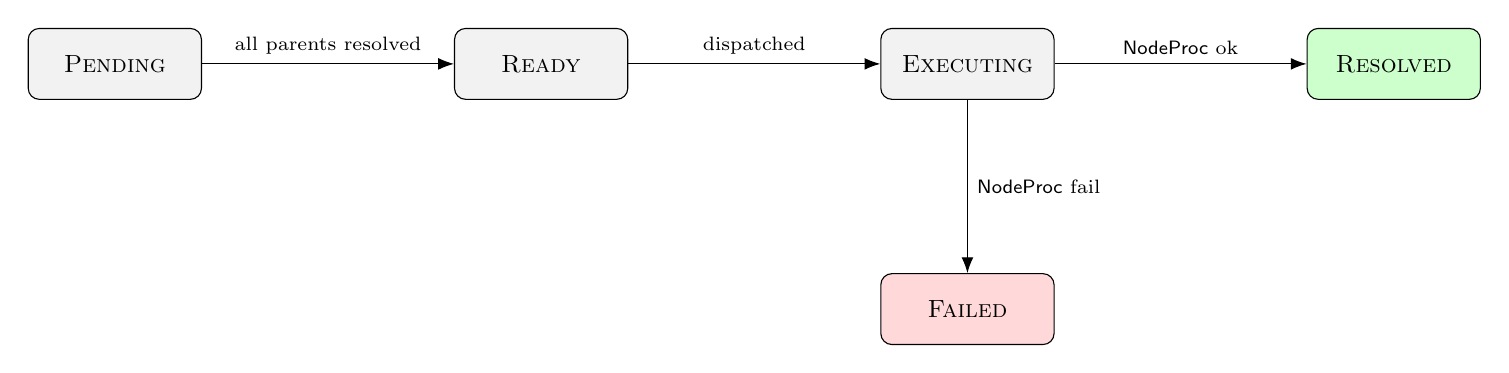
\begin{tikzpicture}[node distance=2.2cm and 3.2cm, every node/.style={font=\small}]
\node[draw,rounded corners,minimum width=2.2cm,minimum height=0.9cm,fill=gray!10] (P) {\PENDING};
\node[draw,rounded corners,minimum width=2.2cm,minimum height=0.9cm,fill=gray!10,right=of P] (R) {\READY};
\node[draw,rounded corners,minimum width=2.2cm,minimum height=0.9cm,fill=gray!10,right=of R] (E) {\EXEC};
\node[draw,rounded corners,minimum width=2.2cm,minimum height=0.9cm,fill=green!20,right=of E] (Re) {\RESOLVED};
\node[draw,rounded corners,minimum width=2.2cm,minimum height=0.9cm,fill=red!15,below=of E] (F) {\FAILED};

\draw[-{Latex[length=2mm]}] (P) -- node[above,font=\scriptsize]{all parents resolved} (R);
\draw[-{Latex[length=2mm]}] (R) -- node[above,font=\scriptsize]{dispatched} (E);
\draw[-{Latex[length=2mm]}] (E) -- node[above,font=\scriptsize]{$\NodeProc$ ok} (Re);
\draw[-{Latex[length=2mm]}] (E) -- node[right,font=\scriptsize]{$\NodeProc$ fail} (F);
\end{tikzpicture}
\caption{The \GSRE\ node-state machine. A node may transition $\PENDING \to \READY$ only when all of its parents are in $\RESOLVED$; $\READY \to \EXEC$ when the scheduler dispatches it; and $\EXEC \to \RESOLVED$ or $\EXEC \to \FAILED$ depending on the outcome of the node-processor call. In the absence of a backtracking policy (Track 1), $\FAILED$ is an absorbing terminal state of the graph.}
\label{fig:state-machine}
\end{figure}

\Cref{fig:state-machine} depicts the transition relation. The key structural fact is that $\PENDING \to \READY$ is gated by a hard predicate on parent state, not by a learned signal: the architecture itself enforces the argument-availability invariant.

\subsection{The traversal engine}

The traversal engine drives the state machine. At each step, it identifies all currently ready nodes, batches them, calls the shared node processor on each, and updates state accordingly. \Cref{alg:gsre} gives the formal pseudocode.

\begin{algorithm}[t]
\caption{The Graph-Structured Recurrent Executor (\GSRE)}
\label{alg:gsre}
\begin{algorithmic}[1]
\Require Well-formed N-DAG $G = (V, r)$ with leaf assignment $\sigma$; node processor $\NodeProc_\theta$.
\Ensure A (possibly partial) value assignment $v : V \rightharpoonup \Val$.
\State \textbf{for each} $n \in V$: $\NState(n) \gets \PENDING$
\State \textbf{for each} leaf $n \in V$: $v_n \gets \sigma(n)$;\; $\NState(n) \gets \RESOLVED$
\Loop
  \State $R \gets \bigl\{n \in V : \NState(n) = \PENDING \text{ and all } p \in \Parents_n \text{ have } \NState(p) = \RESOLVED\bigr\}$
  \State \textbf{for each} $n \in R$: $\NState(n) \gets \READY$
  \If{$R = \emptyset$}
    \If{$\NState(r) = \RESOLVED$} \State \Return $v$
    \ElsIf{$\NState(r) = \FAILED$ \textbf{or} no $\PENDING$ node has all-$\RESOLVED$ parents} \State \Return $v$ \Comment{stuck}
    \EndIf
  \EndIf
  \State $\mathcal{B} \gets R$ \Comment{the \GSRE\ batches all ready nodes for this step}
  \State \textbf{for each} $n \in \mathcal{B}$ (in parallel): $\NState(n) \gets \EXEC$
  \State $\hat{v}_\mathcal{B} \gets \NodeProc_\theta\bigl(\{(\tau_n, \Spec_n, (v_p)_{p \in \Parents_n}) : n \in \mathcal{B}\}\bigr)$
  \For{$n \in \mathcal{B}$}
    \If{$\hat{v}_{\mathcal{B},n} \ne \bot$}
      \State $v_n \gets \hat{v}_{\mathcal{B},n}$;\; $\NState(n) \gets \RESOLVED$
    \Else
      \State $\NState(n) \gets \FAILED$
    \EndIf
  \EndFor
\EndLoop
\end{algorithmic}
\end{algorithm}

Two structural facts are immediate from \Cref{alg:gsre}.

\begin{lemma}[Local Input Determinism]
\label{lem:local-input}
At line~14 of \Cref{alg:gsre}, the input to $\NodeProc_\theta$ for any $n \in \mathcal{B}$ consists exclusively of $\tau_n$, $\Spec_n$, and the resolved values of $\Parents_n$. In particular, this input does not depend on the identity, types, depths, or values of any other node in the graph except via the parent values themselves.
\end{lemma}

\begin{proof}
By inspection of line~14.
\end{proof}

\begin{lemma}[Argument-Availability Invariant]
\label{lem:arg-avail}
At any point in the execution of \Cref{alg:gsre}, if $n$ enters state $\EXEC$ then $\NState(p) = \RESOLVED$ for every $p \in \Parents_n$.
\end{lemma}

\begin{proof}
Transition into $\EXEC$ occurs only at line~13, which is reached only for $n \in \mathcal{B} \subseteq R$, where $R$ was constructed at line~4 to satisfy precisely the predicate that all parents of $n$ are in $\RESOLVED$. Since resolved values are immutable after they are set (line~17), this predicate continues to hold at line~13.
\end{proof}

\subsection{Core operational theorems}

We now state and prove four foundational properties of \GSRE.

\begin{theorem}[Determinism]
\label{thm:gsre-determinism}
Let $\NodeProc_\theta$ be a deterministic function of its input set. Then \Cref{alg:gsre} is a deterministic algorithm: for any well-formed N-DAG $G$ and any leaf assignment $\sigma$, the value assignment $v$ returned by the algorithm is uniquely determined by $G$, $\sigma$, and $\theta$.
\end{theorem}

\begin{proof}
We prove that the value $v_n$ at every node is uniquely determined. Induction on $\dep(n)$.

\emph{Base ($\dep(n) = 0$).} Leaves have $v_n = \sigma(n)$ assigned at line~2 of \Cref{alg:gsre}, which depends only on the input.

\emph{Step.} Let $\dep(n) > 0$ and suppose every $p \in \Parents_n$ has its value uniquely determined. Because $G$ is a DAG and there is no cycle, $n$ eventually appears in the ready set $R$ at some iteration (we will prove termination separately in \Cref{thm:gsre-termination}). At the moment it does, line~12 batches $n$ with other ready nodes. Line~14 calls $\NodeProc_\theta$ with input consisting solely of $\tau_n$, $\Spec_n$, and $(v_p)_{p \in \Parents_n}$ (\Cref{lem:local-input}). These inputs are uniquely determined by $G$, $\sigma$, and $\theta$: $\tau_n$ and $\Spec_n$ from $G$, and the parent values by the inductive hypothesis. Determinism of $\NodeProc_\theta$ then fixes $v_n$ uniquely.

The choice of batch composition $\mathcal{B}$ at line~12 does not affect any node's input by \Cref{lem:local-input}; the same input is presented regardless of which other ready nodes happen to be batched alongside $n$. Hence the value assignment is uniquely determined.
\end{proof}

\begin{theorem}[Order Independence of \GSRE]
\label{thm:gsre-order}
Under the hypothesis of \Cref{thm:gsre-determinism}, the value assignment $v$ produced by \GSRE\ is invariant to the order in which ready nodes are dispatched. That is, if line~12 of \Cref{alg:gsre} is replaced by an arbitrary nonempty subset $\mathcal{B} \subseteq R$ at each iteration, the eventual value assigned to every node that ever becomes $\RESOLVED$ is unchanged.
\end{theorem}

\begin{proof}
The proof of \Cref{thm:gsre-determinism} establishes that the input to $\NodeProc_\theta$ at a node $n$ is independent of which other nodes are batched alongside it. Hence the output value is the same regardless of batch composition.

Furthermore, every node that can ever become $\RESOLVED$ in some schedule does so in every schedule, by the following argument: the set of nodes reachable in $\RESOLVED$ depends only on which nodes ever have all parents simultaneously $\RESOLVED$. This is a property of the parent relation, not of the schedule: under a deterministic node processor that never returns $\bot$, every non-leaf node eventually has all parents resolved (induction on depth). When $\NodeProc_\theta$ may return $\bot$, the set of failed nodes is determined by which nodes' values land on $\bot$, which is itself a function of the (order-independent) inputs.
\end{proof}

\Cref{thm:gsre-order} is conceptually important: it says that the inductive bias of \GSRE\ is genuinely the one we want---the architecture commits only to dependency-respecting execution, not to any particular traversal order.

\begin{theorem}[Termination]
\label{thm:gsre-termination}
\Cref{alg:gsre} terminates in at most $|V|$ iterations of the main loop. In particular, the number of $\NodeProc_\theta$ invocations is at most $|V| - |V_{\mathrm{leaf}}|$.
\end{theorem}

\begin{proof}
At each iteration, at least one node transitions from $\PENDING$ to $\READY$ (line~5), provided $R \ne \emptyset$. We argue this is always the case until either $r$ is $\RESOLVED$ or every $\PENDING$ node has at least one $\FAILED$ ancestor.

Consider the iteration when $r$ is not yet resolved and no node has failed. Define the \emph{frontier} $F = \{n \in V : \NState(n) = \PENDING\}$. Among $F$, the nodes whose parents are all in $V \setminus F = \{n : \NState(n) = \RESOLVED \text{ or } \EXEC\}$ form a nonempty set (this is the standard fact that any nonempty subset of a finite DAG containing at least one descendant-closed element has a minimal element under the induced order, applied to $F$). These minimal elements are exactly $R$, which is therefore nonempty.

Thus each iteration either (i) resolves at least one node (when $R \ne \emptyset$), (ii) fails at least one node (which also reduces $|F|$ by removing it from consideration via the stuck check at lines 7--10), or (iii) returns. After at most $|V|$ iterations, every node has been processed.

Per-node, $\NodeProc_\theta$ is called at most once, so the total number of invocations is at most $|V|$. Leaves are not processed (their values are assigned by line~2), so the bound is in fact at most $|V| - |V_{\mathrm{leaf}}|$.
\end{proof}

\begin{theorem}[Soundness Against the Oracle]
\label{thm:gsre-soundness}
Let $\NodeProc_\theta$ be a deterministic node processor that is \emph{primitive-correct}: that is, for every primitive $\tau \in \Lib$ and every typed input tuple $(v_1, \dots, v_{k_\tau})$, the output of $\NodeProc_\theta$ at any node of type $\tau$ with parent values $(v_1, \dots, v_{k_\tau})$ equals $f_\tau(v_1, \dots, v_{k_\tau})$. Then for any well-formed N-DAG $G$ with leaf assignment $\sigma$, the value $v_r$ returned by \GSRE\ equals the oracle ground-truth answer of \Cref{def:reasoning-task}.
\end{theorem}

\begin{proof}
By induction on $\dep(n)$ together with \Cref{lem:oracle-order}.

\emph{Base.} For a leaf $n$, both \GSRE\ and the oracle assign $v_n = \sigma(n)$.

\emph{Step.} Let $\dep(n) > 0$ and assume that for every $p \in \Parents_n$ the \GSRE\ value $v_p$ equals the oracle value $\hat{v}_p$. By primitive correctness of $\NodeProc_\theta$, the \GSRE\ output at $n$ is $f_{\tau_n}(v_{p_1}, \dots, v_{p_{k_{\tau_n}}}) = f_{\tau_n}(\hat{v}_{p_1}, \dots, \hat{v}_{p_{k_{\tau_n}}}) = \hat{v}_n$.

Applying the induction to $n = r$ gives $v_r = \hat{v}_r$.
\end{proof}

\Cref{thm:gsre-soundness} clarifies the role of the node processor: \emph{the only way \GSRE\ can be wrong is if the node processor is wrong on some primitive in the graph}. This is the source of the capacity--depth decoupling we develop in \Cref{sec:information}.

\subsection{The node processor as a learning target}

The node processor $\NodeProc_\theta$ is a small Transformer (in Track 1, two layers, approximately 2M parameters). Its input at a node $n$ consists of a type embedding for $\tau_n$, a spec encoding for $\Spec_n$, and the resolved values of the parents $\Parents_n$ formatted with type-aware delimiters. Its output is a value of type $\mathsf{out}_{\tau_n}$, produced through a type-appropriate head (regression for numeric types, classification for finite types, copy for string types).

Crucially:
\begin{itemize}[topsep=0pt,itemsep=2pt]
  \item The node processor has no access to any global graph embedding.
  \item It has no access to the index or depth of the node it is processing.
  \item It has no access to a history vector summarising prior nodes.
  \item It is invoked once per node per inference, regardless of where that node sits in the graph.
\end{itemize}

This is what we mean by \emph{local context}: the node processor's input is a function only of the primitive type, the spec, and the parent values. The implications of this design for generalisation are taken up in \Cref{sec:generalization}.

\section{Architectural Comparison: \texorpdfstring{$B_4$}{B4}-tied and \texorpdfstring{$B_5$}{B5} Baselines}
\label{sec:arch-comparison}

The \GSRE\ alone does not give us a useful claim. We need a baseline whose comparison with \GSRE\ isolates the contribution of explicit dependency scheduling. The Track 1 design specifies two natural choices, and the present section formalises them.

\subsection{The \texorpdfstring{$B_4$}{B4}-tied baseline}
\label{sec:b4tied}

\begin{definition}[$B_4$-tied: Weight-Tied Graph Transformer with Causal Ancestor Masking]
\label{def:b4tied}
Let $G = (V, r)$ be a well-formed N-DAG with $|V| = N$. Fix a topological ordering $\pi : V \to \{1, \dots, N\}$, e.g., depth-first preorder. The $B_4$-tied baseline computes node values via $T$ stacked layers, all sharing the same parameters $\theta$:
\begin{align*}
h^{(0)}_n &= \mathsf{Embed}(\tau_n, \Spec_n) \quad \text{for each } n \in V, \\
h^{(t+1)}_n &= \mathsf{Layer}_\theta\!\Bigl(h^{(t)}_n;\; \{h^{(t)}_{n'} : n' \in \mathsf{Ancestors}_\pi(n)\}\Bigr), \quad t = 0, \dots, T-1, \\
v_n &= \mathsf{Head}_{\mathsf{out}_{\tau_n}}\!\bigl(h^{(T)}_n\bigr),
\end{align*}
where $\mathsf{Ancestors}_\pi(n) = \{n' : \pi(n') < \pi(n)\}$, $\mathsf{Layer}_\theta$ is a self-attention block restricted by an ancestor mask, and $\mathsf{Head}_\sigma$ is a type-specific output head.
\end{definition}

The defining structural features of $B_4$-tied are: (i) the per-layer parameters $\theta$ are shared across $t$, yielding weight tying analogous to \GSRE's reuse of $\NodeProc_\theta$; (ii) the attention mask in $\mathsf{Layer}_\theta$ restricts each node to attend only to ancestors in the topological order, preserving the causal structure of the DAG; (iii) all node values are computed in $T$ joint passes rather than node-by-node in dependency order.

The third property is the substantive difference from \GSRE. In $B_4$-tied, a node's representation $h^{(t)}_n$ at layer $t > 0$ depends on \emph{layer-$t$ representations of ancestors}, not on the resolved values $v_p$ of parents. There is no architectural enforcement that parent values are computed before child values: the model has $T$ rounds in which to propagate information.

\subsection{The \texorpdfstring{$B_5$}{B5} baseline}
\label{sec:b5}

\begin{definition}[$B_5$: Sequence Transformer Over the Serialised DAG]
\label{def:b5}
Let $G = (V, r)$ be a well-formed N-DAG. Let $\mathsf{Serialize}(G)$ be a canonical token sequence representation of $G$: for each node in topological order, emit a tuple of tokens encoding its identifier, type, spec, and parent identifiers, separated by delimiters. The $B_5$ baseline computes node values by passing $\mathsf{Serialize}(G)$ through a standard sequence transformer (decoder-only autoregressive, or encoder--decoder) and producing values via type-specific heads at the positions corresponding to each node.
\end{definition}

For the present analysis the architectural details of $B_5$ are immaterial; what matters is that $B_5$ has the same information available as \GSRE\ and $B_4$-tied, but presented as a flat token sequence with no explicit DAG structure.

\subsection{Expressivity containment}

\begin{proposition}[Expressivity Containment]
\label{prop:containment}
For every choice of \GSRE\ parameters $\theta_{\GSRE}$ there exists a choice of $B_4$-tied parameters $\theta_{B_4}$ and depth $T \ge \dep(G)$ such that for every well-formed N-DAG $G$ with depth at most $T$, the value assignment produced by \GSRE\ with $\theta_{\GSRE}$ equals the value assignment produced by $B_4$-tied with $\theta_{B_4}$.
\end{proposition}

\begin{proof}[Proof sketch]
Set $T \ge \dep(G)$. Design the $B_4$-tied layer so that, at layer $t$, a node $n$ with $\dep(n) = t$ first attends to its parents (already resolved at layer $t$ by the inductive construction), copies their values into its working state, and applies $\NodeProc_{\theta_{\GSRE}}$ to compute its own value. At all layers $t' > t$ the node passes its value through unchanged. The ancestor mask permits this attention pattern because parents are ancestors. Crucially, this construction uses the freedom to design layer behaviour as a function of node depth, which can itself be inferred from the masking pattern and position.

Conversely, $B_4$-tied has degrees of freedom that \GSRE\ does not: nothing in the architecture prevents a layer from blending in information from non-parent ancestors, nor from updating a node's representation based on layer-$t$ values of nodes whose true semantic values have not yet been computed (because those nodes' parents are still ``in flight'' at layer $t$). These additional functions are realisable by $B_4$-tied but not by \GSRE.
\end{proof}

\Cref{prop:containment} encodes the key intuition: \GSRE\ is a strictly more constrained function class than $B_4$-tied. This is a feature, not a bug. The hypothesis under test is whether the strict constraint (dependency-respecting computation) is a sufficiently helpful inductive bias to outweigh the loss in expressivity.

\subsection{The inductive-bias differential}

We summarise the differences in a single table. Let $L$ denote the maximum length of the value-encoding tokens for any single resolved value, $N$ the number of nodes in the graph, $d$ the depth of the graph, and $k$ the maximum in-degree of any primitive.

\begin{center}
\begin{tabular}{lccc}
\toprule
\textbf{Property} & \textbf{\GSRE} & \textbf{$B_4$-tied} & \textbf{$B_5$} \\
\midrule
Per-node input length & $\mathcal{O}(k L)$ & $\mathcal{O}(N L)$ via attention & $\mathcal{O}(N L)$ (full seq) \\
Parameters/depth & shared, fixed & shared, fixed & shared, fixed \\
Dependency enforcement & hard, gated & soft, learned & soft, learned \\
Sees node identity & no & yes, via position & yes, via position \\
Sees graph topology & only via parent values & yes, via mask & yes, via tokens \\
\bottomrule
\end{tabular}
\end{center}

\section{Information-Theoretic Analysis}
\label{sec:information}

In this section we make precise two claims about \GSRE: (i) its per-step memory budget is bounded by the maximum in-degree of any primitive, independent of the depth of the graph; and (ii) under a primitive-accurate node processor with per-primitive error rate $\eps$, the executor produces the correct root value with probability at least $(1-\eps)^d$ for a depth-$d$ graph. We refer to these results collectively as \emph{capacity--depth decoupling}.

\subsection{Per-step information budget}

Let $\mathsf{Enc} : \Val \to \{0,1\}^*$ be a fixed encoding of values into bit strings, and let $|\mathsf{Enc}(v)|$ denote the length of the encoding of $v$. Define the \emph{primitive description length} of a node $n$ as
\[
\ell(n) \;=\; |\mathsf{Enc}(\tau_n)| + |\mathsf{Enc}(\Spec_n)| + \sum_{p \in \Parents_n} |\mathsf{Enc}(v_p)|.
\]

\begin{proposition}[Per-Step Bounded Input]
\label{prop:per-step-bounded}
The input length of the node processor at any node $n$ is exactly $\ell(n)$, and
\[
\ell(n) \;\le\; |\mathsf{Enc}(\tau_n)| + |\mathsf{Enc}(\Spec_n)| + k_{\tau_n} \cdot \max_{v \in \Val} |\mathsf{Enc}(v)|.
\]
In particular, if $k_{\max} := \max_{\tau \in \Lib} k_\tau$ and $L_{\max} := \max_{v \in \Val} |\mathsf{Enc}(v)|$ are both finite, then the per-step input length is bounded by $\mathcal{O}(k_{\max} L_{\max})$, independent of $|V|$ and $\dep(G)$.
\end{proposition}

\begin{proof}
The input enumeration follows from the construction of the node-processor call at line~14 of \Cref{alg:gsre}; \Cref{lem:local-input} guarantees that no other content appears in the input. The bound follows by replacing each parent value's encoding by the worst case.
\end{proof}

By contrast, $B_5$ has per-step input of length $\Theta(N L_{\max})$ (the entire serialised DAG), and $B_4$-tied's per-layer attention is over all ancestors, which in the worst case is $\Omega(d)$ nodes per layer. Per-step computational cost is therefore qualitatively different across the three architectures.

\subsection{Capacity--depth decoupling}

We now make explicit the consequence of bounded per-step input for depth scaling.

\begin{theorem}[Capacity--Depth Decoupling under i.i.d. Primitive Error]
\label{thm:capacity-depth}
Let $\NodeProc_\theta$ be a stochastic node processor whose error events at distinct primitive invocations are independent. Let $\eps$ be a uniform upper bound on the probability that $\NodeProc_\theta$ returns a value different from the oracle $f_{\tau_n}$ at any single node (conditional on receiving the oracle parent values). Then for any well-formed N-DAG $G = (V, r)$ of depth $d$ with no shared subexpressions on the path to $r$,
\[
\Prob\bigl[v_r = \hat{v}_r\bigr] \;\ge\; (1-\eps)^{|V| - |V_{\mathrm{leaf}}|} \;\ge\; (1-\eps)^d \cdot \delta(G),
\]
where $\delta(G)$ accounts for non-path nodes and is $\delta(G) = (1-\eps)^{|V| - |V_{\mathrm{leaf}}| - d}$. The per-step parameter count of $\NodeProc_\theta$ remains constant in $d$.
\end{theorem}

\begin{proof}
The event $v_r = \hat{v}_r$ is implied by the joint event that every internal node $n$ satisfies $v_n = \hat{v}_n$. Conditional on all internal nodes having received the correct parent values (i.e., on every parent being correctly resolved), each internal node's $\NodeProc_\theta$ call independently produces the correct value with probability at least $1 - \eps$. Iterating, we obtain
\[
\Prob\bigl[v_n = \hat{v}_n \text{ for all internal } n\bigr] \;\ge\; (1-\eps)^{|V|-|V_{\mathrm{leaf}}|},
\]
which implies the first inequality. The second follows by separating out the at-most-$d$ internal nodes on the path from the lowest leaf to $r$ from the rest.

The claim about per-step parameter count is immediate: $\NodeProc_\theta$ is the same network at every node, with parameter count independent of $|V|$ and $d$.
\end{proof}

\Cref{thm:capacity-depth} is a positive result for \GSRE: if you can drive the per-primitive error rate $\eps$ low enough, depth growth degrades performance gracefully---geometrically, not catastrophically---and at no cost in parameters.

\begin{remark}[Why the same theorem does not hold for $B_5$]
\label{rem:b5-no-decoupling}
A sequence transformer trained on length-$L_{\mathrm{train}}$ serialised DAGs and tested on length-$L_{\mathrm{test}}$ DAGs faces three coupled problems: (i) positional extrapolation, since position embeddings must address indices not seen during training~\cite{press2021train}; (ii) attention dispersion, since the per-step input is longer and the attention weights spread~\cite{anil2022exploring}; (iii) loss of independence between primitive evaluations, since the model is computing all node values in a coupled latent computation. There is no analogue of \Cref{thm:capacity-depth} for $B_5$, and indeed empirically $B_5$-like models degrade non-geometrically with length~\cite{schwarzschild2021can}.
\end{remark}

\begin{remark}[Why the same theorem holds only conditionally for $B_4$-tied]
\label{rem:b4tied-conditional-decoupling}
$B_4$-tied does have shared parameters across layers, and depth in the architectural sense (number of layers $T$) is decoupled from depth in the graph sense (longest path $d$) only if $T \ge d$. If $T$ is fixed at training time, $B_4$-tied will fail to produce correct values for graphs of depth $> T$ regardless of training, because the architecture has insufficient layers to propagate information through. Even with sufficient $T$, $B_4$-tied's per-step computation involves attention over $\Omega(d)$ ancestors per layer, which is qualitatively the same length-extrapolation problem as $B_5$ faces, albeit mitigated by the ancestor mask.
\end{remark}

\section{Generalisation Theory}
\label{sec:generalization}

We now turn to the central question: under what conditions can a model trained on shallow graphs be expected to generalise to deeper graphs? The answer for \GSRE\ is clean; the answer for the baselines is conditional on properties that may not hold.

\subsection{Setup: training and test distributions}

Let $\mathcal{G}_d$ denote the set of well-formed N-DAGs over $\Lib$ of depth exactly $d$, and let $\mathcal{D}_d$ be a probability distribution over $\mathcal{G}_d$ together with a leaf-value distribution. The Track 1 design fixes $\mathcal{D}_{\mathrm{train}} = \frac{1}{3}\sum_{d=1}^{3}\mathcal{D}_d$ and considers test distributions $\mathcal{D}_d$ for $d \in \{1,2,3,4,5,7,9,10\}$. Depths $1$--$3$ are in-distribution; depths $4$--$10$ are out-of-distribution along the depth axis.

\subsection{Local context invariance}

The structural fact about \GSRE\ that yields its generalisation guarantee is invariance to depth at the level of the node processor's input.

\begin{definition}[Local Context]
\label{def:local-context}
The \emph{local context} of a node $n$ in a well-formed N-DAG $G$ with leaf assignment $\sigma$ is the tuple
\[
\mathsf{Ctx}(n) \;=\; \bigl(\tau_n,\; \Spec_n,\; (v_p)_{p \in \Parents_n}\bigr).
\]
\end{definition}

\Cref{lem:local-input} states that the node-processor input at $n$ equals $\mathsf{Ctx}(n)$. Consequently:

\begin{proposition}[\GSRE\ Sees Only Local Contexts]
\label{prop:gsre-local-only}
Let $G$, $G'$ be two well-formed N-DAGs with nodes $n \in G$ and $n' \in G'$ such that $\mathsf{Ctx}(n) = \mathsf{Ctx}(n')$ (equality of types, specs, and parent value tuples). Then the values produced by \GSRE\ at $n$ and $n'$ are identical.
\end{proposition}

\begin{proof}
Immediate from \Cref{lem:local-input} and the determinism of $\NodeProc_\theta$.
\end{proof}

\Cref{prop:gsre-local-only} has a powerful consequence for OOD generalisation:

\begin{theorem}[Local-Context OOD Generalisation]
\label{thm:local-context-ood}
Let $\mathcal{D}_{\mathrm{train}}$, $\mathcal{D}_{\mathrm{test}}$ be two distributions over well-formed N-DAGs, and let $\mathcal{M}_d$ denote the marginal distribution over local contexts $\mathsf{Ctx}(n)$ induced by drawing a graph from $\mathcal{D}_d$ and then drawing an internal node uniformly. If $\mathcal{M}_{\mathrm{train}} = \mathcal{M}_{\mathrm{test}}$, then the per-node error rate of the \GSRE\ node processor is the same under $\mathcal{D}_{\mathrm{train}}$ and $\mathcal{D}_{\mathrm{test}}$.
\end{theorem}

\begin{proof}
The per-node error of the node processor is a function only of $\mathsf{Ctx}(n)$. The expected per-node error under a graph distribution is the integral of this function against $\mathcal{M}_d$. If the marginals agree, the expected errors agree.
\end{proof}

\Cref{thm:local-context-ood} is the formal statement of why \GSRE\ is designed to generalise to deeper graphs: depth shows up in the depth of the DAG and in the number of times the node processor is invoked, but not in the per-invocation marginal distribution of local contexts, so long as the leaf values, types, and specs are drawn from comparable distributions.

\subsection{The OOD generalisation gap}

Combining \Cref{thm:capacity-depth} and \Cref{thm:local-context-ood} yields a clean expression for the expected exact-match accuracy of \GSRE\ as a function of depth.

\begin{corollary}[OOD Accuracy under Local-Context Marginal Invariance]
\label{cor:ood-accuracy}
Under the hypotheses of \Cref{thm:capacity-depth} and \Cref{thm:local-context-ood}, the expected exact-match accuracy of \GSRE\ on a depth-$d$ test distribution $\mathcal{D}_d$ satisfies
\[
\mathrm{Acc}_{\mathcal{D}_d}(\GSRE) \;\ge\; \E_{G \sim \mathcal{D}_d}\Bigl[(1-\eps)^{|V_G| - |V_{G,\mathrm{leaf}}|}\Bigr].
\]
\end{corollary}

\begin{proof}
\Cref{thm:local-context-ood} guarantees that the per-node error rate at any node, including those in test graphs of unfamiliar depth, is bounded above by the training per-node error rate $\eps$. The chain of independent primitive evaluations from \Cref{thm:capacity-depth} then bounds the joint correctness probability.
\end{proof}

For Track 1's chain-shaped graphs of depth $d$ with no shared subexpressions and no degenerate constant-only sub-paths, $|V_G| - |V_{G,\mathrm{leaf}}| = d$, so the lower bound simplifies to $(1-\eps)^d$.

\subsection{Failure modes of the baselines}

Why might $B_4$-tied or $B_5$ fail to exhibit the same depth invariance?

\paragraph{$B_4$-tied: ancestor scope grows with depth.} While $B_4$-tied is constrained to attend only to ancestors, the number of ancestors of a node grows with depth. At a depth-$d$ node in a chain, the ancestor set has size $\Theta(d)$. The attention computation aggregates over this set, and the marginal distribution of \emph{attention input sets} under $\mathcal{D}_d$ shifts with $d$. Unlike \GSRE, $B_4$-tied does not have a fixed-size per-step input.

\paragraph{$B_5$: full sequence length grows.} The serialised DAG length grows with $|V|$, which grows with $d$. Sequence position embeddings, attention dispersion, and softmax temperature interact with the sequence length in well-documented ways~\cite{press2021train, anil2022exploring}.

In both cases the marginal distribution of inputs to the network shifts with depth, so the local-context invariance argument breaks down. Whether the breakdown is empirically significant is exactly what Track 1 measures.

\subsection{Constants vs.\ propagation errors}

A technical caveat to \Cref{thm:local-context-ood}: the assumption that $\mathcal{M}_{\mathrm{train}} = \mathcal{M}_{\mathrm{test}}$ requires control over the value distributions of resolved parents at depth $d$. If primitive functions induce non-uniform value distributions on their outputs (e.g., the modular sum of two uniform values is uniform, but the modular product is not), the marginal value distributions at depth-$d$ nodes will differ from those at depth-$1$ nodes. This is the technical reason the Track 1 design fixes a uniform leaf-value range and uses prime-modulus arithmetic: it preserves the marginal distribution of intermediate values, holding $\mathcal{M}_d$ approximately constant in $d$.

\begin{remark}[Why a prime modulus]
\label{rem:prime-modulus}
For modular arithmetic over $\mathbb{Z}/p\mathbb{Z}$ with $p$ prime, $(\mathbb{Z}/p\mathbb{Z})^\times$ is a cyclic group of order $p-1$. The induced distribution on outputs of $\mathsf{ADD\_MOD}$, $\mathsf{SUB\_MOD}$, and $\mathsf{MUL\_MOD}$ from independent uniform inputs on $\mathbb{Z}/p\mathbb{Z}$ is itself uniform on $\mathbb{Z}/p\mathbb{Z}$ (or on $(\mathbb{Z}/p\mathbb{Z})^\times$ for multiplicative cases conditioned on nonzero inputs). Hence $\mathcal{M}_d$ is approximately invariant in $d$.
\end{remark}

\section{The Track 1 Experimental Hypothesis}
\label{sec:track1}

We now state the Track 1 hypothesis in formal language, and articulate the conditions under which the experiment falsifies it.

\subsection{Formal hypothesis}

\begin{hypothesis}[Track 1 Main]
\label{hyp:track1}
There exists a positive constant $c > 0$ such that, holding training compute, parameter count, and primitive coverage constant, the expected OOD generalisation slope of \GSRE\ across depths $\{5, 7, 9, 10\}$ is at least $c$ greater than that of $B_4$-tied across the same depths.
\end{hypothesis}

The \emph{OOD generalisation slope} is defined as
\[
\mathrm{Slope}(\mathcal{A}) \;=\; \frac{\sum_{d \in \{5,7,9,10\}} \mathrm{Acc}_{\mathcal{D}_d}(\mathcal{A})}{4} \;-\; \mathrm{Acc}_{\mathcal{D}_3}(\mathcal{A}),
\]
where $\mathcal{A}$ is the trained model and $\mathrm{Acc}_{\mathcal{D}_d}(\mathcal{A})$ denotes its exact-match accuracy on the depth-$d$ evaluation set. A more positive slope means more graceful degradation with depth.

\subsection{Decision rules}

\begin{itemize}[topsep=2pt,itemsep=2pt]
  \item If $\mathrm{Slope}(\GSRE) - \mathrm{Slope}(B_4\text{-tied}) > c$ with $95\%$ confidence over 5 seeds, \Cref{hyp:track1} is \textbf{supported}.
  \item If the difference is statistically indistinguishable from zero, the null hypothesis is \textbf{not rejected}: implicit propagation through weight-tied attention masking may be sufficient, and explicit scheduling provides no measurable additional benefit.
  \item If the difference is negative, \Cref{hyp:track1} is \textbf{refuted}, and the explicit scheduling architecture imposes a measurable cost relative to its closest implicit counterpart. This outcome would be a meaningful contribution: it would suggest that the benefits of dependency structure are already captured by ancestor masking in a weight-tied transformer.
\end{itemize}

\subsection{Ablations as causal probes}

The Track 1 design supplements the primary comparison with three ablations:
\begin{itemize}[topsep=2pt,itemsep=2pt]
  \item \textbf{$B_4$ unshared} vs.\ \textbf{$B_4$-tied} isolates the contribution of weight tying within the implicit-propagation family.
  \item \textbf{\GSRE-unshared} vs.\ \textbf{\GSRE} isolates the contribution of weight tying within the explicit-scheduling family.
  \item \textbf{$B_5$} vs.\ \textbf{$B_4$-tied} isolates the contribution of dependency-aware attention masking.
\end{itemize}

Together with the primary comparison \GSRE\ vs.\ $B_4$-tied, the four pairwise contrasts span the design space of (dependency scheduling) $\times$ (weight tying) $\times$ (DAG-aware input).

\section{Track 2: A Reinforcement-Learning Formalisation}
\label{sec:track2}

In Track 2 the oracle expansion grammar is removed: the system must construct the reasoning DAG itself from a known primitive library. We formalise this as a Markov decision process and discuss its structural properties.

\subsection{The graph-construction MDP}

\begin{definition}[Graph-Construction MDP]
\label{def:gcmdp}
The graph-construction MDP for a task specification $q$ over library $\Lib$ is the tuple $(\mathcal{S}, \mathcal{A}, P, R, \gamma)$:

\textbf{State.} $\mathcal{S}$ is the set of pairs $(G, q)$ where $G$ is a partial well-formed N-DAG over $\Lib$ together with a partial value assignment $v$, and $q$ is the task specification. The initial state $s_0$ is $(\emptyset, q)$.

\textbf{Action.} An action is a triple $a = (n_{\mathrm{select}}, \tau, b)$:
\begin{itemize}[topsep=2pt,itemsep=2pt]
  \item $n_{\mathrm{select}}$ is either a $\PENDING$ node with unsatisfied arguments in $G$ (an \emph{expansion target}), or a fresh node identifier (a \emph{new sub-goal}). The first action is necessarily a new sub-goal targeting the task output.
  \item $\tau \in \Lib$ is a primitive whose output type matches the demanded type at $n_{\mathrm{select}}$.
  \item $b$ is a binding of each of $\tau$'s input slots to either an existing resolved value in $G$'s value pool, or a new sub-goal node of the demanded type.
\end{itemize}
A special action $a = \texttt{FAIL}$ terminates the episode.

\textbf{Transition.} $P((G, q), a)$ deterministically produces a new graph $G'$ that incorporates the chosen primitive and bindings, and runs the \GSRE\ traversal engine to resolve any newly-ready nodes. Note that the transition is itself a partial execution of the underlying \GSRE.

\textbf{Reward.} $R(s, a, s')$ is $0$ unless $s'$ contains a fully-resolved root whose value matches the task's ground-truth answer, in which case $R = +1$. \texttt{FAIL} yields $R = 0$.

\textbf{Discount.} $\gamma \in (0, 1)$.
\end{definition}

A policy $\pi : \mathcal{S} \to \Delta(\mathcal{A})$ defines a distribution over actions in each state. The \emph{Graph Policy Network} (\GPN) parameterises such a policy.

\subsection{Action space cardinality}

\begin{proposition}[Per-Step Action Space Size]
\label{prop:action-cardinality}
At a state $s = (G, q)$ with $m$ unfilled slots across all $\PENDING$ nodes and $v$ resolved values in the value pool, the number of legal actions is bounded by
\[
|\mathcal{A}(s)| \;\le\; (m + 1) \cdot |\Lib| \cdot (v + |\Lib|)^{k_{\max}} \;+\; 1,
\]
where the last $+1$ accounts for $\texttt{FAIL}$.
\end{proposition}

\begin{proof}
Choose an expansion target: $m + 1$ options (existing slot or new root subgoal). Choose a primitive: at most $|\Lib|$ options (typically far fewer once type matching is enforced). For each of the up to $k_{\max}$ input slots of the chosen primitive, bind to either an existing resolved value ($v$ choices) or a new sub-goal of the required type ($|\Lib|$ choices, taking primitives as type proxies). Multiplying gives the bound.
\end{proof}

For Track 2's initial linear-chain setting with $|\Lib| \approx 15$, $k_{\max} = 2$, $m \approx 1$ (a single open slot at a time), and $v$ growing modestly through the episode, this is a manageable per-step action space of order $10^2$ to $10^3$, well within the regime of standard RL algorithms.

\subsection{Sample complexity considerations}

The sparse reward structure---$+1$ only on a correctly resolved root---creates the central challenge of Track 2. Two mitigations are anticipated.

\paragraph{Behaviour-cloning bootstrap.} For depths $1$--$3$, where Track 1's oracle expansion grammar produces ground-truth DAGs, the \GPN\ can be pre-trained by supervised learning on the oracle trajectories. The resulting policy serves as the initial distribution for subsequent reinforcement learning. Formally, the bootstrapping loss is
\[
\mathcal{L}_{\mathrm{BC}}(\pi_\phi) \;=\; -\E_{(s,a^\star) \sim \mathcal{D}_{\mathrm{oracle}}}\bigl[\log \pi_\phi(a^\star \mid s)\bigr],
\]
where $a^\star$ is the oracle expansion action at $s$.

\paragraph{MCTS-augmented training.} At inference and during data collection, the \GPN's policy and value head can be used as priors for a Monte Carlo tree search over expansion sequences~\cite{silver2018general}. The MCTS-improved policy targets become the training signal for $\pi_\phi$, in the style of AlphaZero. Because action transitions are deterministic (\Cref{def:gcmdp}), MCTS over the graph-construction MDP is particularly clean: every rollout is a no-stochasticity simulation of the executor, and value estimates depend only on the leaf policy and the (deterministic) executor.

\begin{remark}[Why deterministic transitions matter]
\label{rem:det-transitions}
In stochastic-transition MDPs, MCTS rollouts conflate policy improvement with environment variance reduction. In the graph-construction MDP, the only randomness is in the policy itself; once the policy is fixed and the random seed of any stochastic node processor is fixed, the trajectory is deterministic. This makes the MCTS-AlphaZero recipe a particularly natural fit.
\end{remark}

\subsection{Risks and partial mitigations}

The risks already identified in the proposal map onto concrete formal concerns:

\begin{itemize}[topsep=2pt,itemsep=2pt]
  \item \textbf{Sparse reward.} With $+1$-only reward, the credit-assignment problem is severe even for depth $5$. The mitigations enumerated above (BC bootstrap, MCTS) address this in principle. Adding dense intermediate signals (e.g., reward per correctly-resolved intermediate node) is possible but biases the policy toward greedy expansion and is therefore an avenue of last resort.
  \item \textbf{Scalability.} \Cref{prop:action-cardinality} shows the per-step action space is bounded by $(m+1)|\Lib|(v+|\Lib|)^{k_{\max}}$. For general DAGs with high in-degree and many open slots, this grows quickly. Track 2 deliberately restricts attention to chain-shaped tasks; general DAGs are deferred.
  \item \textbf{Dependence on $\NodeProc_\theta$.} The graph-construction MDP's transition function calls the node processor to resolve newly-ready nodes. A node processor with error rate $\eps$ will inject noise into the transition itself, blurring the policy's view of the value pool. Track 1's characterisation of $\eps$ as a function of training depth informs the Track 2 design.
\end{itemize}

\section{Track 3: The Formal Obstacles to Primitive Invention}
\label{sec:track3}

Track 3 envisions a system that autonomously extends its own primitive library. This is unsolved territory. The purpose of the present section is not to propose a solution, but to articulate the open problems in language that connects to standing research in program synthesis, library learning, and continual learning.

\subsection{Subgraph abstraction}

The first formal problem is the identification of reusable subgraphs in successful traces. Let $\mathcal{T} = \{G_1, G_2, \dots\}$ be a collection of successfully-resolved N-DAGs. A \emph{subgraph abstraction} is a typed parameterised graph template $T$ and an embedding mapping $\iota_i : T \hookrightarrow G_i$ for each $G_i \in \mathcal{T}_T \subseteq \mathcal{T}$, such that $\iota_i$ preserves the structure of $T$ up to substitution of free type variables and leaves.

\begin{definition}[Compositional Compression]
\label{def:compression}
A subgraph abstraction $T$ \emph{compresses} the trace collection $\mathcal{T}$ by an amount
\[
\Delta(T) \;=\; \sum_{i : T \hookrightarrow G_i} \bigl(|T_{\mathrm{instances in } G_i}| - 1\bigr) \cdot |T| \;-\; |T|,
\]
i.e., the bits saved by replacing $T$'s multiple instances with a single abstract reference, minus the cost of storing $T$ itself.
\end{definition}

The search problem is to find $T$ with high $\Delta(T)$. This is closely related to graph mining and pattern frequency~\cite{washio2003state}, to program library learning in DreamCoder~\cite{ellis2021dreamcoder}, and to the wake-sleep methodology of inductive program synthesis. The challenge specific to \NBRS\ is that subgraph templates must be parameterised by \emph{types}, not just by constants, and the type system permits open type variables in the input slots of the abstracted primitive.

\subsection{Continual learning of the node processor}

Adding a new primitive $\tau_{K+1}$ to the library requires the node processor $\NodeProc_\theta$ to learn it. Continual learning of a shared multi-task transformer is a known hard problem.

\begin{conjecture}[Compositional Continual Learning is Possible]
\label{conj:ccl}
For a shared node processor $\NodeProc_\theta$ trained on a sequence of primitives $\tau_1, \tau_2, \dots$ each constructed by abstraction from successful traces involving previously-learned primitives, there exists a training schedule and a parameter-regularisation scheme under which (i) the per-primitive accuracy on each $\tau_i$ remains above $1 - \eps$ for some uniform $\eps > 0$; and (ii) the time to reach $1 - \eps$ accuracy on $\tau_{K+1}$ is sublinear in $K$.
\end{conjecture}

We are unaware of any general technique that achieves both (i) and (ii) for shared transformer architectures. Approaches in the recent literature---LoRA-style adapters~\cite{hu2021lora}, elastic-weight consolidation~\cite{kirkpatrick2017overcoming}, mixture-of-experts---each give up one of these properties for the other. Reconciling them is an open problem and a precondition for Track 3.

\subsection{Verification of invented primitives}

If a new primitive $\tau_{K+1}$ is induced from data, the system must verify that it computes a useful function. Two interpretations of ``useful'' are possible:

\begin{itemize}[topsep=2pt,itemsep=2pt]
  \item \textbf{Compression-based verification.} The new primitive is useful if including it in the library reduces the description length of held-out problem solutions by a margin exceeding the cost of carrying its parameters.
  \item \textbf{Semantic verification.} The new primitive must compute a well-defined mathematical function $f_{\tau_{K+1}}$. Without an external oracle, this function is implicit in the parameters of $\NodeProc_\theta$, and ``correctness'' is whatever the node processor produces.
\end{itemize}

Compression-based verification is realisable and is the metric DreamCoder uses. Semantic verification raises a foundational question: \emph{can the system construct test cases for its own invented primitives?} In principle, abstracted primitives come with example traces from the corpus they were mined from, and these examples can serve as a self-generated test set. In practice, the test set defines correctness, and the system has no separate ground truth.

\subsection{Search vs.\ abstraction}

When confronted with a novel problem, the system can either (i) attempt to solve it by search over existing primitives, or (ii) attempt to introduce a new primitive. The choice involves meta-reasoning that depends on the empirical search cost of (i) and the compression value of (ii). We have no principled treatment of this tradeoff; it remains the most open of the open problems of Track 3.

\subsection{Symbolic-neural interface stability}

A final subtle issue: once the system modifies its own operation schemas, the clean separation between symbolic traversal and neural execution---which is the entire architectural premise---becomes recursive. The traversal engine itself must adapt to new node types it has never seen, and the type system itself may need to extend (new types for new primitive outputs). We expect this recursion to be tractable only by maintaining a fixed type system and restricting primitive invention to be type-conservative (no new types are introduced).

\section{Connections to Prior Work}
\label{sec:related}

The \NBRS\ programme draws on, and connects to, several lines of research.

\paragraph{Length and compositional generalisation.} The SCAN benchmark~\cite{lake2018generalization} and its descendants~\cite{kim2020cogs, hupkes2020compositionality} established the empirical reality of the compositional-generalisation gap. Subsequent work explored architectural variants that close the gap on specific benchmarks: tree-structured input~\cite{russin2019compositional}, transformer architectural modifications~\cite{csordas2021devil}, training-data augmentation~\cite{andreas2020good}. \NBRS\ is in this tradition but addresses compositional generalisation through structural enforcement rather than data augmentation.

\paragraph{Chain-of-thought and scratchpad reasoning.} Wei et al.~\cite{wei2022chain} and Nye et al.~\cite{nye2021show} demonstrated that providing intermediate reasoning steps as targets dramatically improves multi-step task performance. These methods can be viewed as expressing the reasoning DAG implicitly in sequence form. \NBRS\ makes the structure explicit.

\paragraph{Recurrent and universal transformers.} Dehghani et al.~\cite{dehghani2018universal} introduced weight-tied transformers in which the same layer is applied recurrently. \GSRE's \texttt{$B_4$-tied} baseline is a graph-structured analogue. The relationship between weight tying and length generalisation has been investigated empirically by~\cite{schwarzschild2021can}.

\paragraph{Neural module networks.} Andreas et al.~\cite{andreas2016neural} proposed networks whose computation graph is determined by a parse of the input question, instantiating modules from a fixed library. \NBRS\ generalises the underlying idea: the computation graph is an explicit, typed DAG, and the modules are unified into a single shared neural module.

\paragraph{Program synthesis and library learning.} Track 2 is a neural program synthesis problem with a known DSL; the literature is vast~\cite{gulwani2017program, polosukhin2018neural, devlin2017robustfill}. Track 3 is a library learning problem, most closely related to DreamCoder~\cite{ellis2021dreamcoder} and earlier work on inductive program synthesis~\cite{summers1977methodology}. The novelty of \NBRS\ in this space is the hybrid neural-symbolic substrate: a learned node processor backed by an explicit traversal engine.

\paragraph{Graph neural networks.} The $B_4$-tied baseline is structurally related to graph neural networks~\cite{kipf2016semi, velivckovic2017graph}, particularly to message-passing variants. The key difference is that GNN message passing operates without dependency-respecting gating: every node updates at every layer in parallel, regardless of whether its input has stabilised.

\paragraph{Causal masking and order constraints.} Causal attention masking has been used in graph transformers~\cite{dwivedi2020generalization}, but typically to encode a fixed topological order rather than to enforce dependency-respecting execution.

\section{Limitations}
\label{sec:limitations}

We close with a careful enumeration of the limitations of the theoretical framework developed here.

\paragraph{Independence assumption in \Cref{thm:capacity-depth}.} The geometric decay $(1-\eps)^d$ assumed independence of primitive errors across nodes. Empirically, errors at correlated input values (e.g., near-edge cases of modular arithmetic) may be correlated, yielding worse depth scaling. The theorem provides a lower bound under the independence assumption; the actual scaling is an empirical question.

\paragraph{Marginal-invariance assumption in \Cref{thm:local-context-ood}.} The assumption that the marginal distribution of local contexts is preserved across depths requires careful control over leaf-value distributions and primitive choice. The Track 1 design controls these via uniform sampling and prime-modulus arithmetic; in more complex tasks, marginal invariance may fail.

\paragraph{The node-processor error rate $\eps$ may itself grow with depth.} Even though the marginal distribution of local contexts is invariant in depth, the actual training data emphasises shallow contexts. Subtle over-reliance on co-occurring shallow features could yield an $\eps$ that grows with depth. This is what the experimental measurement of OOD slope checks.

\paragraph{The expressivity-containment result (\Cref{prop:containment}) is constructive but not informative about learning.} $B_4$-tied can implement \GSRE, but whether gradient descent in $B_4$-tied parameter space finds the \GSRE-implementing setting is a question about training dynamics, not expressivity. Track 1's empirical setup is precisely a test of this learning question.

\paragraph{The MDP formalisation of Track 2 ignores partial observability.} In a realistic deployment, the task specification $q$ may be ambiguous (e.g., natural-language goals). Resolving the ambiguity is itself a perception problem, and the MDP we wrote down assumes $q$ is given in a fully-specified form.

\paragraph{Track 3 is a research agenda, not a proposal.} The formal language we provided in \Cref{sec:track3} should not be mistaken for a plan to solve the open problems. Each of the four subsections represents a multi-year research direction in its own right.

\paragraph{No discussion of compute cost.} We have not analysed the wall-clock cost of \GSRE\ relative to its baselines. In production deployment, the cost of $|V|$ sequential node-processor invocations may exceed the cost of a single transformer pass on the serialised DAG. Whether the depth-generalisation benefit translates into deployment value depends on the cost ratio and the per-step parallelism achievable on accelerator hardware.

\section{Conclusion}
\label{sec:conclusion}

The Notion-Based Reasoning System rests on a simple structural hypothesis: that reasoning is fundamentally a partial-order computation, and that representing this partial order explicitly---combined with a small recurrent neural module---unlocks compositional depth generalisation that fully-parallel attention architectures struggle to achieve.

We have formalised the central object of the design (the Graph-Structured Recurrent Executor), proved its core operational properties, articulated its expected information-theoretic advantage over implicit-propagation baselines, and stated the Track 1 empirical hypothesis in falsifiable form. We have also formalised the Track 2 reinforcement-learning problem and articulated the open formal problems of Track 3.

Whether the experiment supports or refutes the hypothesis, the value of the framework lies in turning a vague intuition about ``structural reasoning'' into a definite, testable, comparable claim. The success of the programme will be measured not by whether \GSRE\ ``works'', but by what we learn about the interaction between explicit dependency structure and neural function approximation in compositional reasoning.

\paragraph{What changes for the reader.} If Track 1 is supported, we will have evidence that hard architectural enforcement of dependency structure provides measurable benefit over implicit attention-based enforcement. If Track 1 is not rejected, we will have evidence that implicit enforcement is sufficient and the architectural complexity of \GSRE\ is unjustified for this regime. Either outcome is informative; both shape the design choices for Track 2 and the prioritisation among the open problems of Track 3.

\bigskip
\noindent\textbf{Approved for implementation: Track 1.}\\
\noindent\textbf{Tracks 2 and 3 remain exploratory and will be refined based on Track 1 outcomes.}

\bigskip

\appendix

\section{Notation Summary}
\label{app:notation}

\begin{center}
\begin{tabular}{ll}
\toprule
\textbf{Symbol} & \textbf{Meaning} \\
\midrule
$\Types$ & Set of types in the type system. \\
$\Val_\tau$ & Value domain of type $\tau$. \\
$\Lib$ & Primitive library. $|\Lib| = K$. \\
$\tau$ & A primitive operation; $\mathsf{in}_\tau$, $\mathsf{out}_\tau$, $f_\tau$ are its input/output types and semantics. \\
$n$ & A notion: $(\mathsf{id}_n, \tau_n, \Spec_n, \Parents_n)$. \\
$G = (V, r)$ & A notion DAG with vertex set $V$ and root $r$. \\
$\dep(n)$ & Compositional depth of notion $n$. \\
$\dep(G)$ & Depth of the graph; $= \dep(r)$. \\
$\NState(n)$ & Current execution state of $n \in \{\PENDING, \READY, \EXEC, \RESOLVED, \FAILED\}$. \\
$v_n$ & Resolved value at node $n$. \\
$\hat{v}_n$ & Oracle ground-truth value at node $n$. \\
$\NodeProc_\theta$ & Shared neural node processor with parameters $\theta$. \\
$\eps$ & Per-primitive error rate of $\NodeProc_\theta$. \\
$k_{\tau}$ & Arity of primitive $\tau$. $k_{\max} = \max_\tau k_\tau$. \\
$\mathsf{Ctx}(n)$ & Local context of node $n$: $(\tau_n, \Spec_n, (v_p)_{p \in \Parents_n})$. \\
$\mathcal{D}_d$ & Distribution over depth-$d$ N-DAGs. \\
$\mathcal{M}_d$ & Marginal distribution over local contexts under $\mathcal{D}_d$. \\
$\GPN_\phi$ & Graph Policy Network for Track 2, parameters $\phi$. \\
\bottomrule
\end{tabular}
\end{center}

\section{A Worked GSRE Trace}
\label{app:trace}

For concreteness we trace the execution of \GSRE\ on the DAG of \Cref{ex:small-chain}: $((3+5)-2)\cdot 7 \mod 101$.

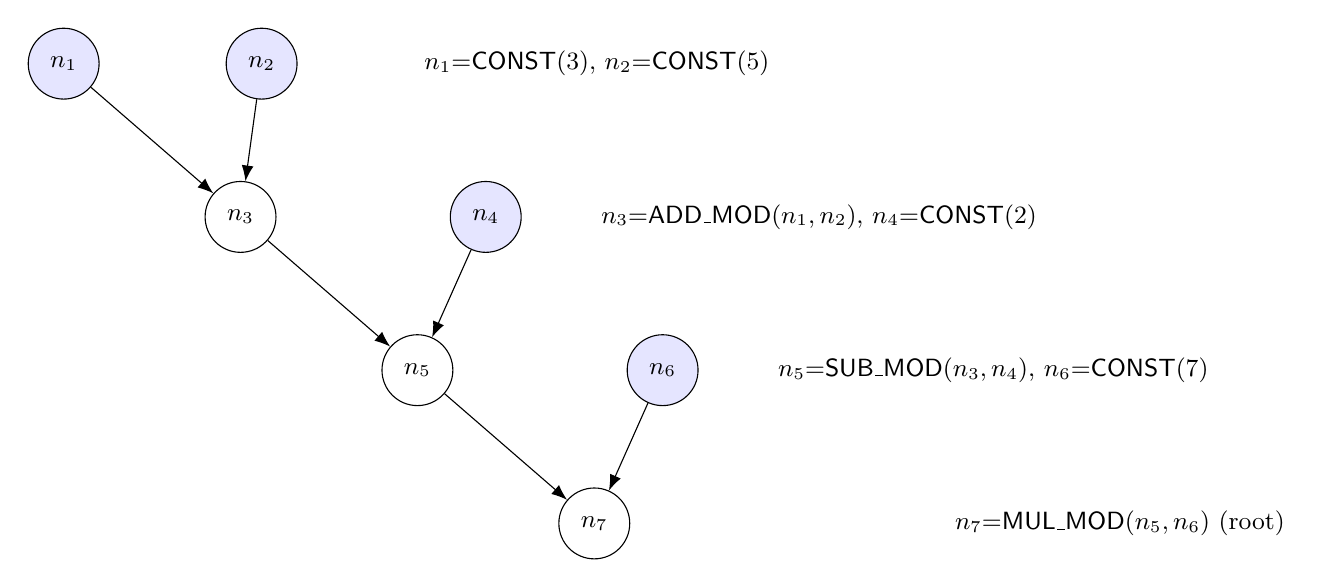
\begin{tikzpicture}[node distance=1.3cm and 1.6cm, every node/.style={font=\small}]
\node[draw,circle,minimum size=0.9cm,fill=blue!10] (n1) {$n_1$};
\node[draw,circle,minimum size=0.9cm,fill=blue!10,right=of n1] (n2) {$n_2$};
\node[draw,circle,minimum size=0.9cm,below right=of n1] (n3) {$n_3$};
\node[draw,circle,minimum size=0.9cm,fill=blue!10,right=2.2cm of n3] (n4) {$n_4$};
\node[draw,circle,minimum size=0.9cm,below right=of n3] (n5) {$n_5$};
\node[draw,circle,minimum size=0.9cm,fill=blue!10,right=2.2cm of n5] (n6) {$n_6$};
\node[draw,circle,minimum size=0.9cm,below right=of n5] (n7) {$n_7$};

\draw[-{Latex[length=2mm]}] (n1) -- (n3);
\draw[-{Latex[length=2mm]}] (n2) -- (n3);
\draw[-{Latex[length=2mm]}] (n3) -- (n5);
\draw[-{Latex[length=2mm]}] (n4) -- (n5);
\draw[-{Latex[length=2mm]}] (n5) -- (n7);
\draw[-{Latex[length=2mm]}] (n6) -- (n7);

\node[right=4cm of n1, font=\small] {$n_1{=}\mathsf{CONST}(3)$, $n_2{=}\mathsf{CONST}(5)$};
\node[right=4cm of n3, font=\small] {$n_3{=}\mathsf{ADD\_MOD}(n_1,n_2)$, $n_4{=}\mathsf{CONST}(2)$};
\node[right=4cm of n5, font=\small] {$n_5{=}\mathsf{SUB\_MOD}(n_3,n_4)$, $n_6{=}\mathsf{CONST}(7)$};
\node[right=4cm of n7, font=\small] {$n_7{=}\mathsf{MUL\_MOD}(n_5,n_6)$ (root)};
\end{tikzpicture}

The execution trace is:
\begin{enumerate}[itemsep=2pt,topsep=2pt]
  \item \emph{Initialisation.} All leaves ($n_1, n_2, n_4, n_6$) are assigned constants and marked $\RESOLVED$ with values $3, 5, 2, 7$ respectively. All other nodes are $\PENDING$.
  \item \emph{Iter 1.} The ready set is $R = \{n_3\}$, since $n_3$'s parents $n_1, n_2$ are both $\RESOLVED$. $\NodeProc_\theta$ is called with input $(\mathsf{ADD\_MOD}, \cdot, (3, 5))$. The output is $8$. $v_{n_3} = 8$, $\NState(n_3) = \RESOLVED$.
  \item \emph{Iter 2.} The ready set is $R = \{n_5\}$. $\NodeProc_\theta$ is called with input $(\mathsf{SUB\_MOD}, \cdot, (8, 2))$. The output is $6$. $v_{n_5} = 6$, $\NState(n_5) = \RESOLVED$.
  \item \emph{Iter 3.} The ready set is $R = \{n_7\}$. $\NodeProc_\theta$ is called with input $(\mathsf{MUL\_MOD}, \cdot, (6, 7))$. The output is $42$. $v_{n_7} = 42$, $\NState(n_7) = \RESOLVED$.
  \item \emph{Termination.} The root $r = n_7$ is $\RESOLVED$, so the loop exits and returns $v$ with $v_r = 42$.
\end{enumerate}

In this trace, $\NodeProc_\theta$ was invoked three times (once per internal node), and at each invocation its input length was bounded by the description length of the primitive plus two parent values---no part of the input depended on the depth of the graph or on the identity of nodes outside the direct parents.

\begin{thebibliography}{99}

\bibitem{lake2018generalization}
B.~M. Lake and M.~Baroni.
Generalization without systematicity: On the compositional skills of sequence-to-sequence recurrent networks.
In \emph{ICML}, 2018.

\bibitem{kim2020cogs}
N.~Kim and T.~Linzen.
COGS: A compositional generalization challenge based on semantic interpretation.
In \emph{EMNLP}, 2020.

\bibitem{hupkes2020compositionality}
D.~Hupkes, V.~Dankers, M.~Mul, and E.~Bruni.
Compositionality decomposed: How do neural networks generalise?
\emph{JAIR}, 67, 2020.

\bibitem{anil2022exploring}
C.~Anil et al.
Exploring length generalization in large language models.
In \emph{NeurIPS}, 2022.

\bibitem{nogueira2021investigating}
R.~Nogueira, Z.~Jiang, and J.~Lin.
Investigating the limitations of transformers with simple arithmetic tasks.
\emph{arXiv:2102.13019}, 2021.

\bibitem{schwarzschild2021can}
A.~Schwarzschild, E.~Borgnia, A.~Gupta, F.~Huang, U.~Vishkin, M.~Goldblum, and T.~Goldstein.
Can you learn an algorithm? Generalizing from easy to hard problems with recurrent networks.
In \emph{NeurIPS}, 2021.

\bibitem{wei2022chain}
J.~Wei et al.
Chain-of-thought prompting elicits reasoning in large language models.
In \emph{NeurIPS}, 2022.

\bibitem{nye2021show}
M.~Nye et al.
Show your work: Scratchpads for intermediate computation with language models.
\emph{arXiv:2112.00114}, 2021.

\bibitem{dehghani2018universal}
M.~Dehghani, S.~Gouws, O.~Vinyals, J.~Uszkoreit, and L.~Kaiser.
Universal transformers.
In \emph{ICLR}, 2019.

\bibitem{press2021train}
O.~Press, N.~A. Smith, and M.~Lewis.
Train short, test long: Attention with linear biases enables input length extrapolation.
In \emph{ICLR}, 2022.

\bibitem{russin2019compositional}
J.~Russin, J.~Jo, R.~C. O'Reilly, and Y.~Bengio.
Compositional generalization in a deep seq2seq model by separating syntax and semantics.
\emph{arXiv:1904.09708}, 2019.

\bibitem{csordas2021devil}
R.~Csord{\'a}s, K.~Irie, and J.~Schmidhuber.
The devil is in the detail: Simple tricks improve systematic generalization of transformers.
In \emph{EMNLP}, 2021.

\bibitem{andreas2020good}
J.~Andreas.
Good-enough compositional data augmentation.
In \emph{ACL}, 2020.

\bibitem{andreas2016neural}
J.~Andreas, M.~Rohrbach, T.~Darrell, and D.~Klein.
Neural module networks.
In \emph{CVPR}, 2016.

\bibitem{gulwani2017program}
S.~Gulwani, O.~Polozov, and R.~Singh.
Program synthesis.
\emph{Foundations and Trends in Programming Languages}, 4(1--2), 2017.

\bibitem{polosukhin2018neural}
I.~Polosukhin and A.~Skidanov.
Neural program search: Solving programming tasks from description and examples.
\emph{arXiv:1802.04335}, 2018.

\bibitem{devlin2017robustfill}
J.~Devlin, J.~Uesato, S.~Bhupatiraju, R.~Singh, A.-R. Mohamed, and P.~Kohli.
RobustFill: Neural program learning under noisy I/O.
In \emph{ICML}, 2017.

\bibitem{ellis2021dreamcoder}
K.~Ellis et al.
DreamCoder: Bootstrapping inductive program synthesis with wake-sleep library learning.
In \emph{PLDI}, 2021.

\bibitem{summers1977methodology}
P.~D. Summers.
A methodology for LISP program construction from examples.
\emph{JACM}, 24(1), 1977.

\bibitem{kipf2016semi}
T.~N. Kipf and M.~Welling.
Semi-supervised classification with graph convolutional networks.
In \emph{ICLR}, 2017.

\bibitem{velivckovic2017graph}
P.~Veli{\v{c}}kovi{\'c} et al.
Graph attention networks.
In \emph{ICLR}, 2018.

\bibitem{dwivedi2020generalization}
V.~P. Dwivedi and X.~Bresson.
A generalization of transformer networks to graphs.
\emph{arXiv:2012.09699}, 2020.

\bibitem{silver2018general}
D.~Silver et al.
A general reinforcement learning algorithm that masters chess, shogi, and Go through self-play.
\emph{Science}, 362(6419), 2018.

\bibitem{hu2021lora}
E.~J. Hu et al.
LoRA: Low-rank adaptation of large language models.
In \emph{ICLR}, 2022.

\bibitem{kirkpatrick2017overcoming}
J.~Kirkpatrick et al.
Overcoming catastrophic forgetting in neural networks.
\emph{PNAS}, 114(13), 2017.

\bibitem{washio2003state}
T.~Washio and H.~Motoda.
State of the art of graph-based data mining.
\emph{ACM SIGKDD Explorations}, 5(1), 2003.

\end{thebibliography}

\end{document}
